\documentclass[lettersize,journal,english]{IEEEtran}
\usepackage[T1]{fontenc}
\usepackage[utf8]{inputenc}
\usepackage{amsmath,amsfonts,amssymb}
% \usepackage{algorithmic}
% \usepackage{algorithm}
\usepackage{array}
\usepackage[caption=false,font=normalsize,labelfont=sf,textfont=sf]{subfig}
\usepackage{textcomp}
\usepackage{stfloats}
\usepackage{url}
\usepackage{verbatim}
\usepackage{graphicx}
\usepackage{cite}
\usepackage{booktabs}
\usepackage{units}
\usepackage[unicode=true,pdfusetitle,
 bookmarks=true,bookmarksnumbered=false,bookmarksopen=false,
 breaklinks=false,pdfborder={0 0 0},pdfborderstyle={},backref=false,colorlinks=true]{hyperref}
\hypersetup{urlcolor=blue, linkcolor=black}

\title{Adaptative neighbouring methods applied to telephonic base stations}
\author{\IEEEauthorblockN{Paul MÉHAUD}\\
\IEEEauthorblockA{\textit{Intern at CTU in Prague} \\
\textit{INSA Rouen Normandie}\\
paul.mehaud@insa-rouen.fr}\\
\and
\IEEEauthorblockN{Brendan SÉVELLEC}\\
\IEEEauthorblockA{\textit{Intern at CTU in Prague} \\
\textit{INSA Rouen Normandie}\\
brendan.sevellec@insa-rouen.fr}}

\usepackage[english,french]{babel}

\begin{document}
\selectlanguage{english}
\maketitle

\begin{abstract}
    Nowadays, it is primordial for telecommunication companies to be able to determine if a user is moving. For that, it is necessary to understand the neighbouring relationships between the telephonic base stations. This article aims at proposing and optimizing a method that adaptively detects these relationship between telephonic base stations. 
    
    This methods consists in multiple steps that can each be realised thanks to several methods that are compared: the $k$-NN method, the Delaunay triangulation or the Gabriel graph method are first used to create a first rough estimation of each point's neighbours. A filtering step is then applied in order to refine the neighbouring relationships that were found. This step is composed of several criteria that are successively being applied. 
    
    These criteria are coming from previous works but were enhanced for better computational cost and results, and also to locally take into account the density of base station in the neighbours computation. 
    
    The resulting method therefore gives a more accurate estimation of the neighbouring relationship than what was proposed before.
\end{abstract}

\begin{IEEEkeywords}
    Neighbours, Telecommunication, Base station, $k$-NN, Adaptative.
\end{IEEEkeywords}
\section{Introduction}
    \IEEEPARstart{T}{he} field of telecommunication represents a gigantic mine of information, the smartphone penetration rate being 69\% in 2023 in the world, and 97\% in France. Therefore, the collected datas represent a big opportunity for telecommunication companies to predict their customers behaviour for internal or marketing purposes. 
    
    This article articulates around the themes of mobile networks and neighbouring problems. 

    A cellular network, also know as a mobile network, is a type of telecommunications network that is dispersed over geographical areas known as cells, each of which is supplied by at least one fixed-location transceiver called base station (BS). These BSs give the cell network coverage so that voice, data, and other kinds of content may be transmitted.
    
    Given a list of points and their coordinates, a neighbouring problem consists in finding, for each point, a list of other points that are considered as its neighbours.

    The field of neighbouring problems mainly revolves around the optimisation of the $k$ Nearest Neighbours ($k$-NN) algorithm.
    As indicated by its name, this method consists in considering the closest $k$ points of each points as their neighbour.
    [insert KNN reference]

    Another method consists in the using the Delauney triangulation. Each couple of points linked by an edge in this triangulation are considered neighbours.
    [insert Delauney neighbouring reference]

    The default of the $k$-NN method is that it always find the same number of neighbours to each point, independantly to the reality of the geometry around each BS.
    
    The Delaunay triangulation seems to solve this issue but it also have its own set of defaults, mostly on the borders of the data where it creates aberrant edges.

    Here two BSs are considered as neighbours if their converage area overlap. Therefore, these generic methods aren't perfectly adapted to this application as these coverage areas are submitted to specific limitations like limitted radius and wave interferences.

    Therefore, some researchs were done in order to adapt these methods to this specific application \cite{patent_neighs}.

    This article aims at enhance the precision of these methods . It also aims at comparing the efficiency of different approaches. 

    Therefore, the outcome of the method presented is a neighbouring graph, cf. Figure~\ref{fig:neigh_graph}, where each node is a BS and each edge represent a neighbouring relationship between these two BSs.
    \begin{figure}
        \centering
        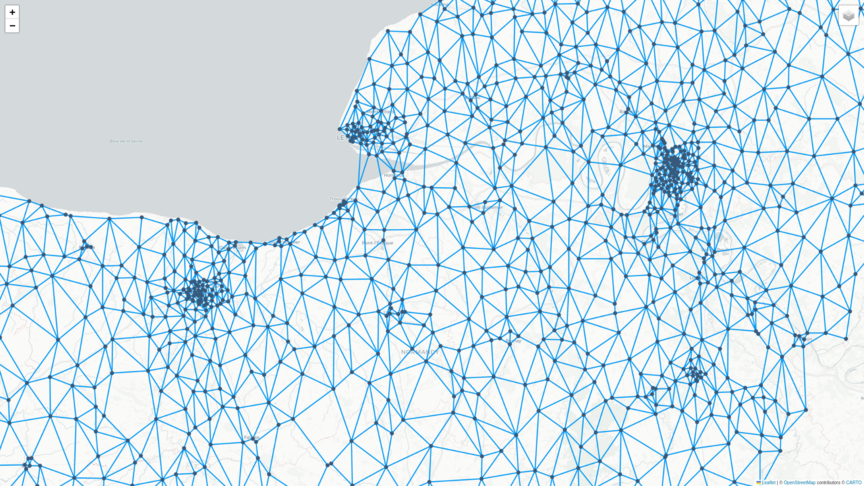
\includegraphics[width=3.5in]{images/illus_graphs/neighbouring_graph.png}
        \caption{Illustration of a neighbouring graph.}
        \label{fig:neigh_graph}
    \end{figure}

    A key finding of this article is to locally take into account the density of BS in the neighbouring methodology.

    The rest of the paper is organized as follows: Section~\ref{sec:rel_works} reviews the related works relevant to our research. In Section~\ref{sec:data}, we detail the databases used in our analysis. Section~\ref{sec:overview} offers an overview existing methods. Section~\ref{sec:contrib} outlines our contributions. In Section~\ref{sec:res}, we present the results, analyzing the performance and implications of our proposed methods. Finally, Section~\ref{sec:ccl} concludes the paper and suggests directions for future research.

\section{Related works\label{sec:rel_works}}
    \noindent 

\section{Databases\label{sec:data}}
    \noindent Several databases have been used in order to test the different aspects of the methods. However, one of them is directly necessary to the method itself.

    \subsection{Main database}
        In this study, this database \cite{main_database} that contains all the information needed for the application of the method is being used. It is from the French Regulatory Authority for Electronic Communications and Posts (ARCEP), which is an independent French administrative authority responsible for regulating electronic and postal communications and press distribution.

        This database was first published for the third quarter of 2017 and the version used here was published on 28\textsuperscript{th} March 2024 \cite{main_database_hist}.
        It's updated for every quarter. For instance, this data refers to the fourth quarter of 2023.

        It consists of a substantial collection of $108\,838$ entries, encompassing $29$ distinct features of a size of $\unit[16.7]{Mo}$.
        Each row of the database corresponds to detailed information regarding a specific BS. For the scope of this study, our analysis is focusing on the fields outlined in Table~\ref{table:data_columns}.
        \begin{table}
            \centering
            \caption{Description of the main database columns used in the experiments.}
            \label{table:data_columns}
            \begin{tabular}{ll}
                \toprule
                \textbf{Column} & \textbf{Description} \\
                \cmidrule(lr){1-2}
                \textsl{id\_station\_anfr} & ANFR BS ID \\ 
                \textsl{nom\_op} & Name of the provider \\
                \textsl{$x$, $y$, latitude, longitude} & Base station coordinates \\ 
                \textsl{nom\_reg, nom\_dep, nom\_com} & Additional location information \\  
                \textsl{site\_2g, 3g, 4g, 5g} & Technology used by the BS \\ 
                \bottomrule
            \end{tabular}
        \end{table}

        For station coordinates, two different reference points are used: $x$ and $y$ coordinates, which are Lambert-93 projections of latitude and longitude.
        This dual system has two advantages: the $x$, $y$ coordinates allow us to calculate distances in meters using the Euclidean norm, which is more efficient in terms of calculation, and the GPS coordinates make it easier to display the points on a map.

        In addition, in the columns the name of the provider (\textsl{nom\_op}) is given.

        Finally, informations about the technologies used in every site is provided. Indeed, a site can use multiple technologies.
        In Figure~\ref{fig:data_evolution} the evolution of each technology from the first updates of the data can be found.
        \begin{figure}
            \centering
            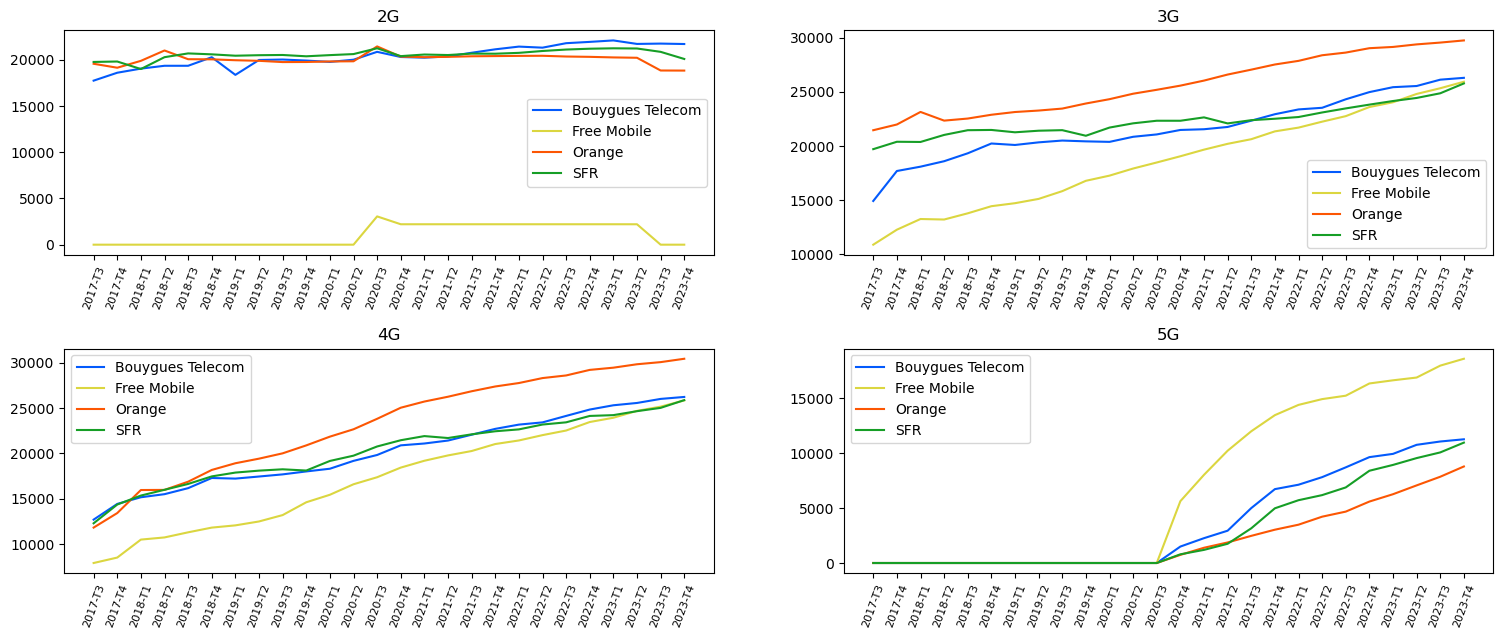
\includegraphics[width=3.5in]{images/data_analysis/technos-evolution.png}
            \caption{Evolution by quarter year and by technology of the number of BS.}
            \label{fig:data_evolution}
        \end{figure}
        Then, in Figure~\ref{fig:data_technos} a chart showing the number of times each technology is present for each provider can be found.
        \begin{figure}
            \centering
            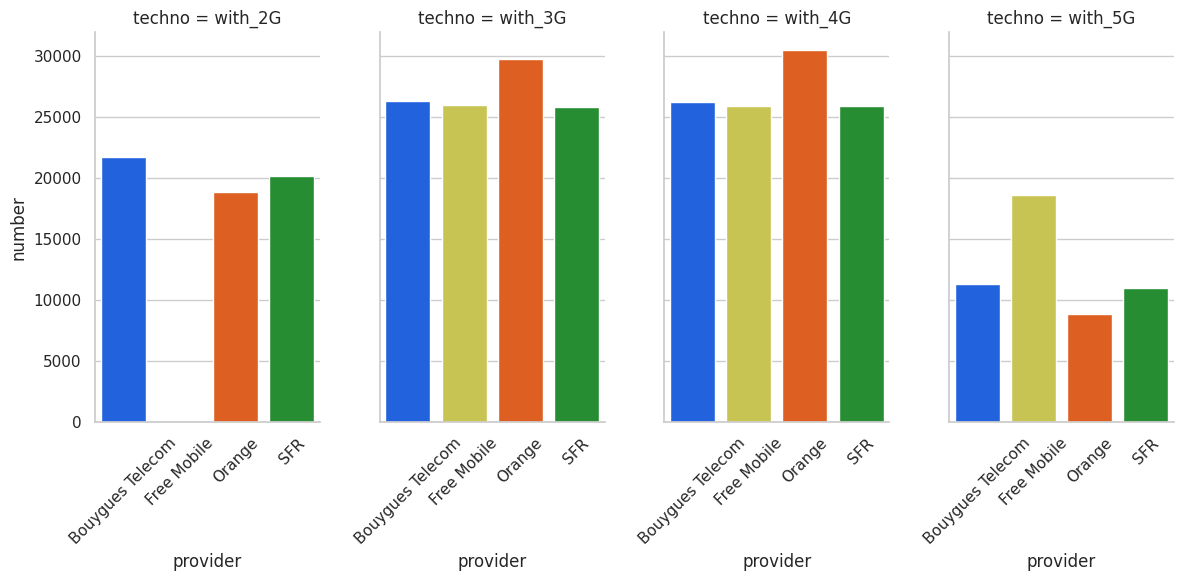
\includegraphics[width=3.5in]{images/data_analysis/with_techno.png}
            \caption{Breakdown, by operator, of the number of sites containing a given technology.}
            \label{fig:data_technos}
        \end{figure}
        We can see, for example, that \emph{Free Mobile} doesn't have any BS with $2$G technology. Additionally, you can also find these values in Table~\ref{table:techno_numbers}.
        \begin{table}
            \centering
            \caption{Number of BS equipped, at least, with $x$G, by provider.}
            \label{table:techno_numbers}
            \begin{tabular}{cccccc}
                \toprule
                \textbf{Technology} & \textbf{Bouygues} & \textbf{Free} & \textbf{Orange} & \textbf{SFR} & \textbf{Total} \\
                \cmidrule(lr){1-6}
                \textbf{2G} & 21710 & 0 & 18835 & 20093 & 60638 \\
                \textbf{3G} & 26294 & 25934 & 29748 & 25777 & 107753 \\
                \textbf{4G} & 26231 & 25847 & 30440 & 25881 & 108399 \\
                \textbf{5G} & 11271 & 18607 & 8794 & 10968 & 49640 \\
                \textbf{Total} & 26331 & 25949 & 30540 & 26018 & 108838 \\
                \bottomrule
            \end{tabular}
        \end{table}

    \subsection{Filtering the main database}
        As seen before this database is really big, as a matter of fact only a portion of it is used.

        Firstly, only one provider is considered because a BS from provider $x$ can't be considered as a neighbour of BS from provider $y$.
        Consequently, we have chosen \emph{Orange} because it is the one that has the largest number of BS.

        Secondly, for the same reasons as before, only one technology is considered. Thus, all BS using, at least, 4G are taken into account.

        In order to simplify the calculation times, the vision and the assessment of the quality of the results, only sites located in the Normandy region are studied.
        This is because Normandy is where our school is based, giving us a better view of its geography.

    \subsection{Additional database}
        In order to compare the results of city detection, a reference database was needed. We therefore used the population data provided by INSEE.
        [Pas sûr de l'utilité de présenter cette base en fait, ptet juste la principale suffit]

\section{Overview of use methods\label{sec:overview}}
    \subsection{Finding potential neighbours}
        When looking for neighbours, at first, a list of potential neighbours for each point is necessary.
        For that, a neighbouring graph is constructed where $P$ is the set of all points and each edge in this graph represents a neighbouring relation.

        \subsubsection{$k$-NN graph}
            The most intuitive method is to connect each point to its $k$ nearest neighbours, where $k \in \mathbb{N}^*$ is a parameter to be set up. 

            However, this method can be questioned, because it always finds $k$ neighbours for each point, no matter the reality of the data.

        \subsubsection{Delaunay triangulation}
            A Delaunay triangulation \cite{art_delaunay} of a set of points in the plane subdivides their convex hull into triangles whose circumcircles do not contain any of the points.

            A Voronoi diagram is a tessellation pattern in which $n$ points scattered on a plane subdivides in exactly $n$ cells enclosing a portion of the plane that is closest to each point. 

            It is a well-known method when trying to find neighbours \cite{delaunay_neighbor} since a Delaunay triangulation is the pendant of a Voronoi diagram, cf. Figure~\ref{fig:del_tri}, i.e. two points are connected in the
            Delaunay triangulation if their associated cells are touching each other in the Voronoi diagram.

            \begin{figure}
                \centering
                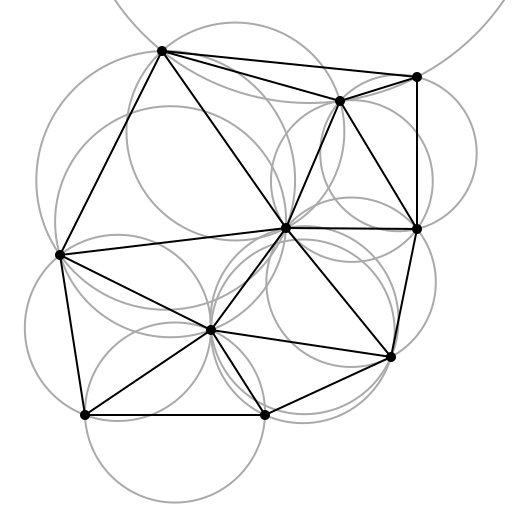
\includegraphics[width=1.6in]{images/illus_graphs/Delaunay_circumcircles_vectorial.png}
                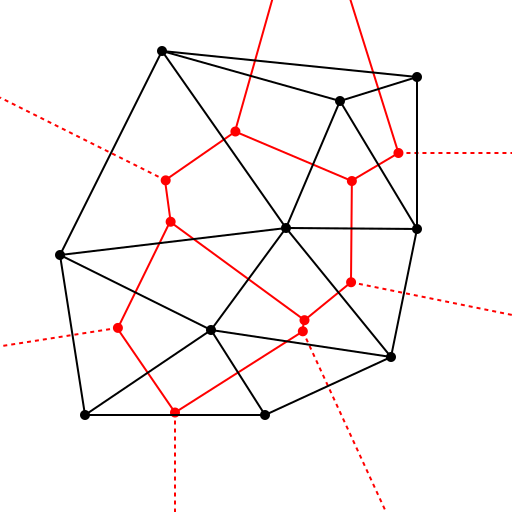
\includegraphics[width=1.6in]{images/illus_graphs/Delaunay_Voronoi.png}
                \caption{Example of a Delaunay triangulation (in black) and Voronoi diagram (in red).}
                \label{fig:del_tri}
            \end{figure}

        \subsubsection{Gabriel graph}
            A Gabriel graph \cite{10.2307/2412323} is a subgraph of a Delaunay triangulation. Thus, if the Delaunay triangulation is given, it can be found in a linear time. 

            Formally, it is the graph in which any two distinct points $p, q \in P$ are adjacent precisely when the closed disc having $pq$ as a diameter contains no other points.

            Basically, the interset of this method, compared to the Delaunay triangulation, is that it is adding a first level of filtration to suppress some neighbouring connexions.

    \subsection{Finding real neighbours}
        For the purpose of our experiments, i.e. finding BS neighbours, the previously presented methods are not sufficient to find real neighbours.
        As a consequence, some neighbouring connexions needs to be suppressed \cite{patent_neighs}.
        \subsubsection{Distance criterion}
            A BS does not have an infinite coverage area.
            As a consequence, each edge in $U$ that is longer than a certain value, called \emph{max\_distance}, is suppressed.

        \subsubsection{Angle criterion}
            Let $p$, $q$, $r$ be three BS of $P$, where $q$ and $r$ are $p$'s potential neighbours. As said before, coverage areas of BS are limited by physics, this also implies that $r$ can be \og hidden\fg{} from $p$ by $q$ because $q$ is between $p$ and $r$ [trouver qqch pour prouver ce que je dis].

            Therefore, the connexion between $p$ and $r$ needs to be suppressed. How? The angle $\widehat{qrp}$ is calculated and if it is narrower than a certain value, called \emph{min\_angle}, the longest edge is suppressed.

        \subsubsection{Quadrant criterion}
            As introduced in a previous article \cite{10201211} its goal is to prevent all potential neighbours to be in the same angle range. Therefore, it was mainly thought to be used with the $k$-NN potential neighbours method.

            It consists in dividing the space around each BS into quadrants and keeping only a certain number of potential neighbours in each of the quadrants, cf. Figure~\ref{fig:crit_qua}.
            The number of quadrants has been fixed to six \cite{art_del_paq}.

    \subsection{Density-based clustering methods}
        \subsubsection{DBScan}
            DBScan consists in detecting clusters based on the density of points, using two parameters:
            \begin{itemize}
                \item $\varepsilon$: A distance threshold under which two points are considered close enough to be considered neighbours;   
                \item $n_{\text{min}}$: The shortest number of neighbours a points needs to have to be considered as a core point of a cluster.
            \end{itemize}

            The clusters are then \og growing\fg{} from the core points by attaching all points close from less than $\varepsilon$ than a point of the said cluster.

        \subsubsection{HDBScan}
            HDBScan \cite{10.1007/978-3-642-37456-2_14} is a variation of the DBScan method.
            It consists in selecting the best clusters after testing their persistence by making the $\varepsilon$ parameter vary. It's main particularity is that it allows to detect clusters of different densities.

            To each point who belongs to a cluster is associated a probability that symbolises the degree of certainty for this point to belong to the said cluster.

\section{Contributions\label{sec:contrib}}
    \noindent In section~\ref{sec:overview}, we have seen that we can find the neighbours of BSs by combining a potential neighbouring graph and filtration criteria. This methodology gives pretty good results \cite{art_del_paq}.

    However, in certain cases like in a city, the filtration criteria aren't precise enough. We, therefore, need to find some ways to measure BSs' density.

    \subsection{Measurement of BS density}
        Places with a high population also have a high density of BSs. In fact, each BS can only support a certain load of users.

        Therefore, let's assume that finding zones with a high density of BS is equivalent to finding the BS situated in \og cities\fg{}.

        \subsubsection{DBScan}
            The most intuitive method to use when trying to locate zones with high a high density of point is DBScan. In fact, by applying the methods with the right parameters, these zones are detected in separate clusters and the rest is considered as noise. Two categories are therefore created: city (all the clusters) and countryside (the noise).

        \subsubsection{HDBScan}
            We can use HDBScan the same way. However, the previously mentionned probability associated with each point belonging to a cluster can be used to separate the center of the city (where the probability is very high) from the rest of the city.

        \subsubsection{$3$-NN mean distance}
            For each BS $p\in P$, the mean distance $\gamma_p$, in $\unit{km}$, to its three nearest neighbours is calculated. According to the value of $\gamma_p$, a BS is classified into a different category of density. In fact, a low $\gamma_p$ means that the surrounding zone is very dense in BS. On the contrary, a high value translate to a low density area (countryside).

            For this method to work properly, only BS from the same provider have to be kept into the calculation process.

    \subsection{Improvement of filtering criteria}

        \subsubsection{Distance and angle criterion}
            As seen in section~\ref{sec:overview}, after having found potential neighbours for each BS, this connexions needs to be filtrated. However, this applies the same distance and angle threshold for all BSs, without taking in account the difference of density.

            The proposesd method is to take into account those differences of density for each site to apply a different threshold according to the category the site in classified in.

            For both distance and angle, the more the BS is in a dense category, the lower this threshold is.

        \subsubsection{Quadrant criterion}
            This criterion has been upgraded by adding the possibility to rotate the quadrants. The offset angle selected, which is between $0$ and $60$ degrees, is the one that maximises the sum of the distances of the potential neighbours to their closest quadrant delimitation.

            In other words, it tends to select the angle with which the potential neighbours are as much in the middle of their respective quadrants as possible.

            The quadrant criterion is illustrated in Fig~\ref{fig:crit_qua}.
            \begin{figure}
                \centering
                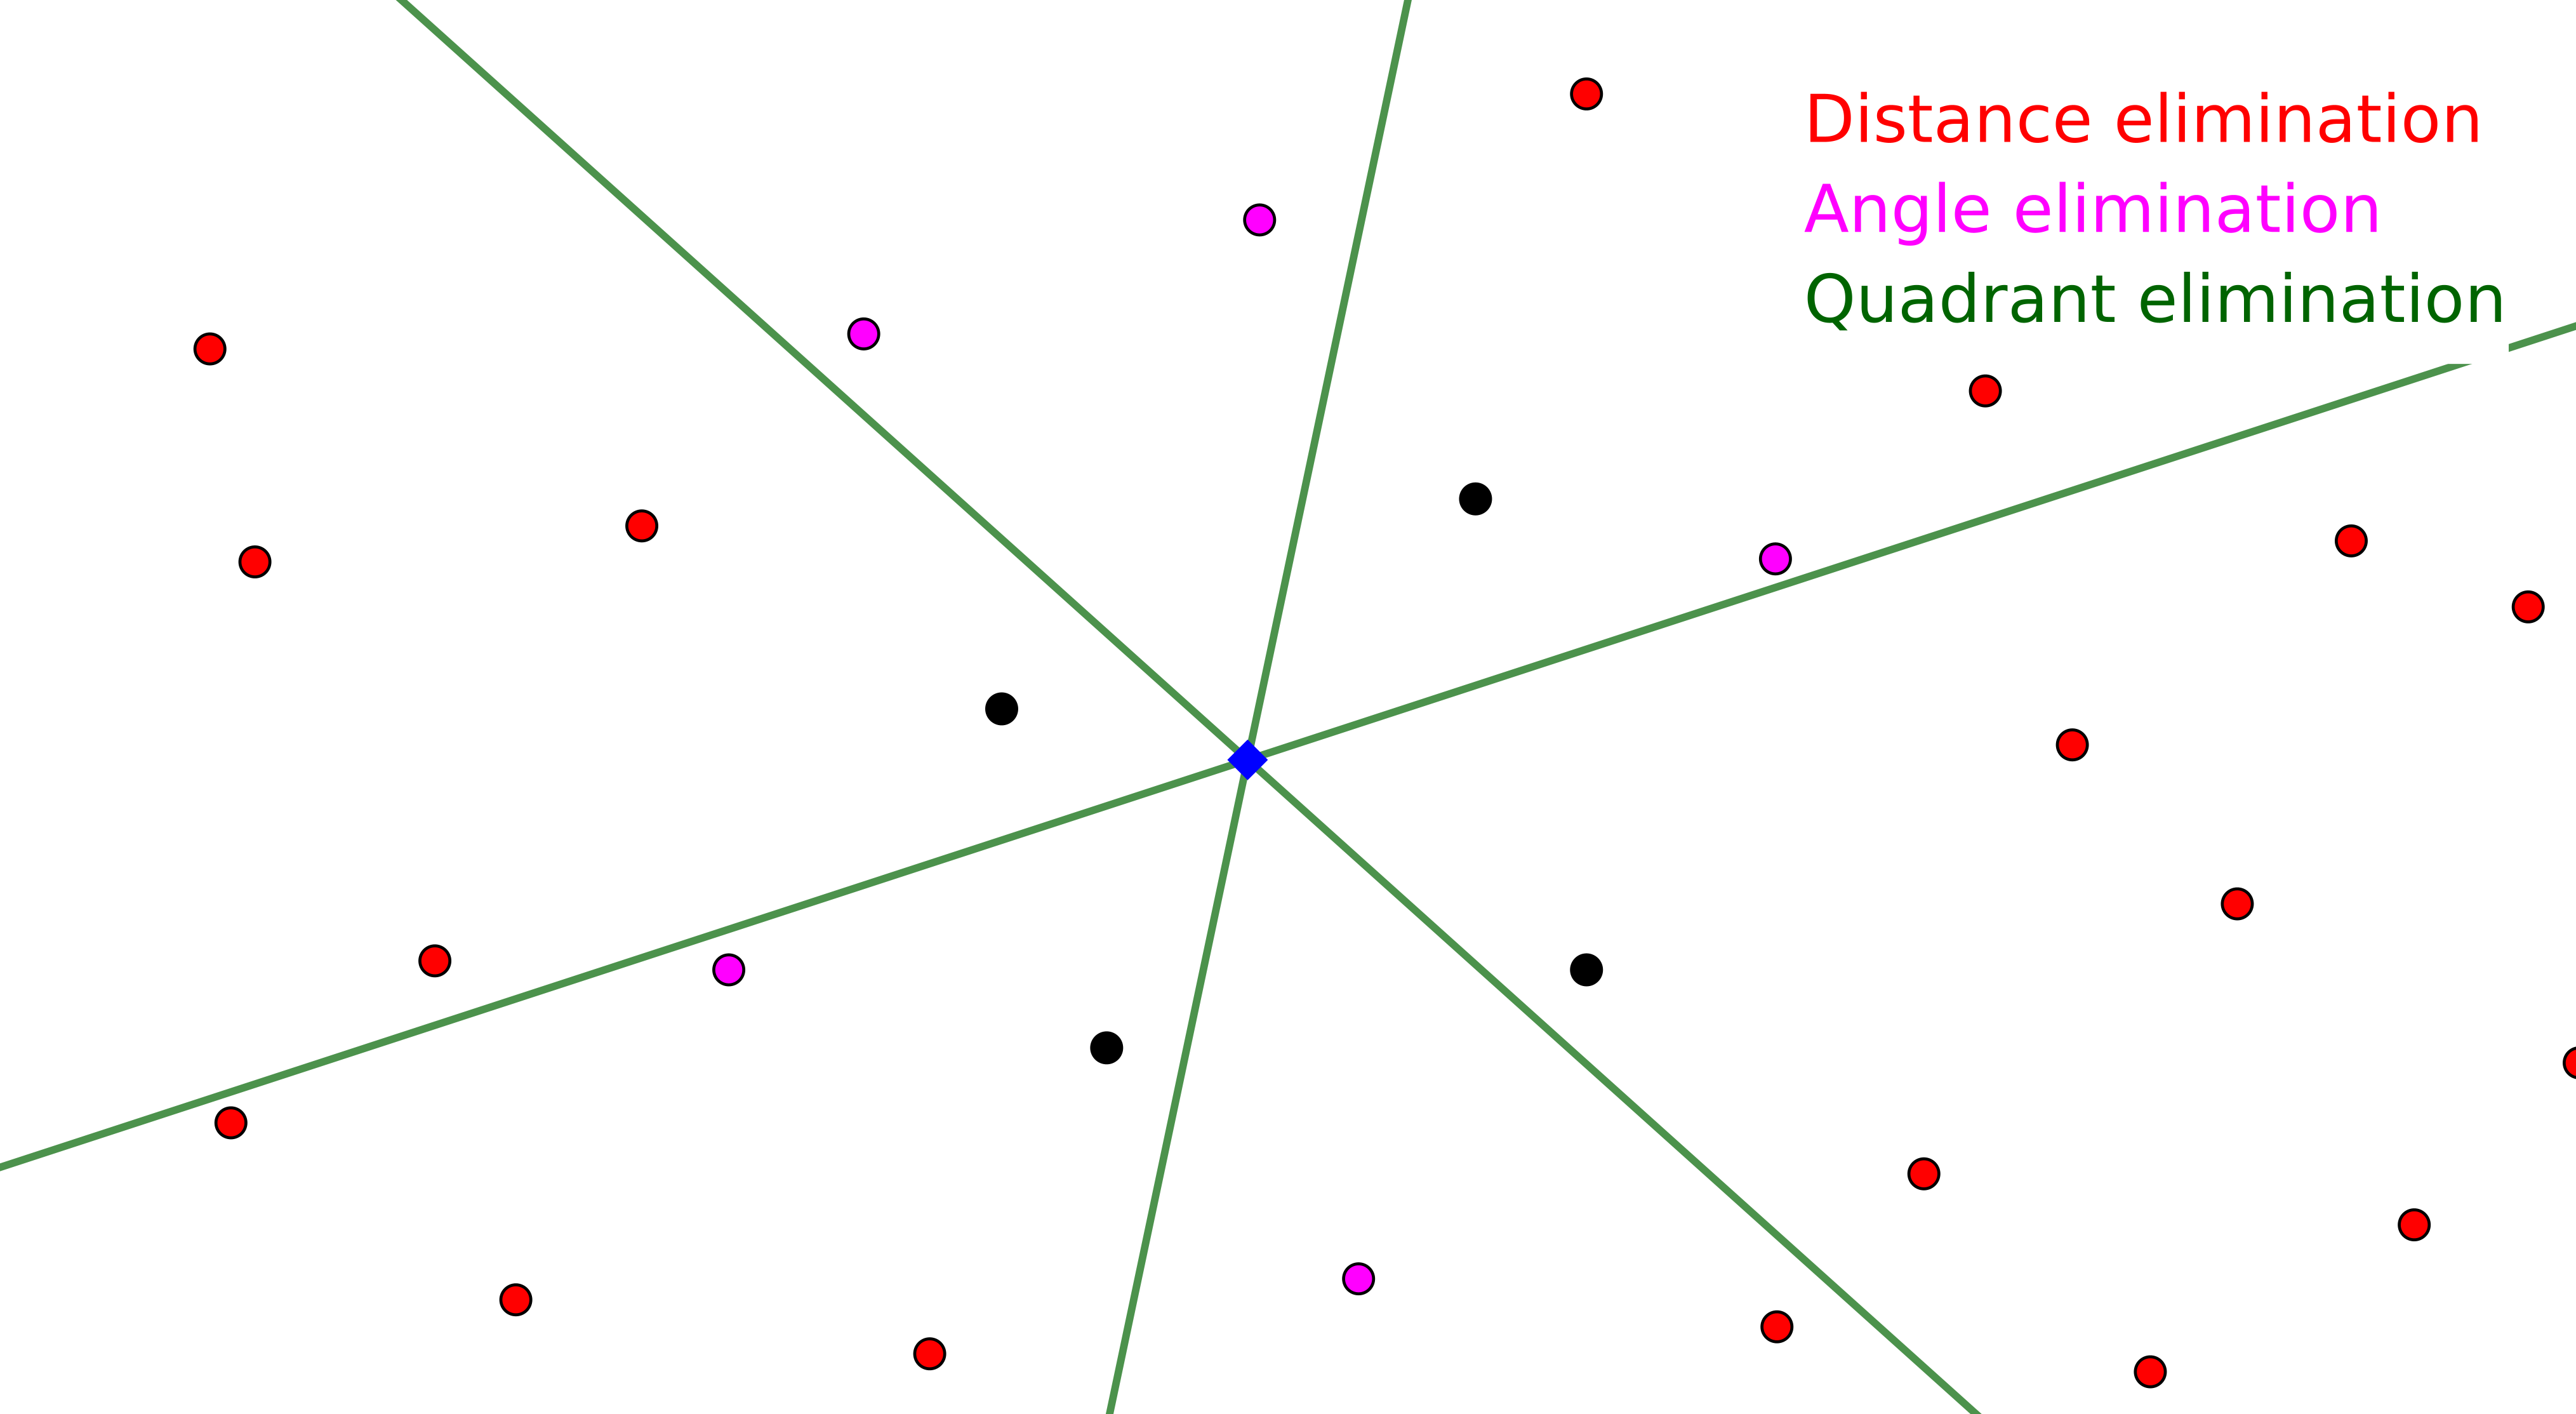
\includegraphics[width=3.5in]{images/illus_crit/quadrant_elim.png}
                \caption{Illustation of the rotated quadrant criterion.}
                \label{fig:crit_qua}
            \end{figure}

\section{Results\label{sec:res}}
    \subsection{Measurement of BS density}
        Each of the three methods for detecting the high density base stations that were described above detect the major cities of France. It is even possible to accurately detect the name of these cities by looking, for each cluster, at the most represented "nom\_com" field of the base station of the cluster.

        Morevover, the correlation coefficient between the number of inhabitant and the number of base station is above 0.9 for each of the methods.

        As seen before, HDBScan is a method of variable density. In this use case, it is a drawback because the density of base station accurately represents the radius of each base station's coverage. It is therefore not advisable to treat each cluster differently. Plus, this method often presents aberrant clusters like the entire Corsica.

        When comparing the cluster detected to the cities that have more than 7000 inhabitants, 3-NN is the method that has the best result. In fact, if we consider all base station with a $\gamma_p$ value inferior to 2 km to be in cities we find that the percentage at accurately classified base station is 88\%. It is 87\% for DBScan and 85\% for HDBScan.

        Plus, as seen before, we can use the $\gamma_p$ value of the 3-NN method to classify each city in precise category, not only city vs coutryside. 

        Here is the classification that has been chosen : 
        \begin{itemize}
            \item city center: $\gamma_p\in [0,1]$;
            \item urban area: $\gamma_p\in ]1,2]$;
            \item extra-urban: $\gamma_p\in ]2,4]$;
            \item countryside: $\gamma_p\in ]4,\infty[$.
        \end{itemize}

    \subsection{Best potential neighbours}
        First of all, the $k$-NN method could have provided a solution to the fact that the Delaunay triangulation does not connect all the points but makes choices. However, to obtain interesting connections, we need to choose a relatively high $k$, greater than 10, which implies a large number of connections and therefore an increase in   computational cost. What's more, applying the criteria doesn't even produce convincing results.
        
        Secondly, the use of Gabriel's graph is not conclusive either. In fact, the use of this type of graph is not appropriate here because it will remove neighbourhood relationships that could have been retained.

        Finally, taking into account the above conclusions, the method used to construct the potential neighbourhood is the Delaunay triangulation.

    \subsection{Optimizing criteria parameters}
        As seen in Section~\ref{sec:contrib}, the angle and distance criteria must adapt their threshold to the density of base station. The chosen thresholds for each of the previously introduced categories are presented in Table~\ref{table:crit_summary}. if both potential neighbours are in a different category, then the higher threshold is chosen.
g
        \begin{table}
            \centering
            \caption{Summary of criteria values.}
            \label{table:crit_summary}
            \begin{tabular}{lcc}
                \toprule
                \textbf{Description} & \textbf{\emph{max\_distance}} & \textbf{\emph{min\_angle}} \\
                \cmidrule(lr){1-3}
                city center & $\unit[2]{km}$ & $5^\circ$ \\
                urban area & $\unit[5]{km}$ & $10^\circ$ \\
                extra-urban area & $\unit[10]{km}$ & $15^\circ$ \\
                countryside & $\unit[15]{km}$ & $20^\circ$ \\
                \bottomrule
            \end{tabular}
        \end{table}
    
        
    \subsection{Combining criteria}
        The accuracy of the results depends on which criteria are applied to potential neighbours, and also on the order in which they are applied.

        Firstly, the tests focused on the various possible combinations of the three criteria. When doing this experiment, the results were really convincing but, sometimes, some connexions were suppressed even if there was no reason to suppress them. In addition, those results were mostly influenced by when the quadrant criterion is applied.

        Consequently, combinations of two criteria were experimented. At that moment, all these unexplained suppressions disappeared, especially when the quadrant criterion wasn't applied.

        Now a choice has to be made between which criterion to apply first: distance or angle? The first option is prefered because it is more optimised. Indeed, the distance criterion takes less of computer ressources, thus reducing the number of operations to treat by the angle criterion.

        In Figure~\ref{fig:final_neighs} you have an illustration of a portion of the results. To clarify, the colour of the points, which represent the BSs, is in function of the $\gamma_p$ value.

        In the future, there will be method to compare our results with a reference. [pas sûr si on garde ca]
        \begin{figure}
            \centering
            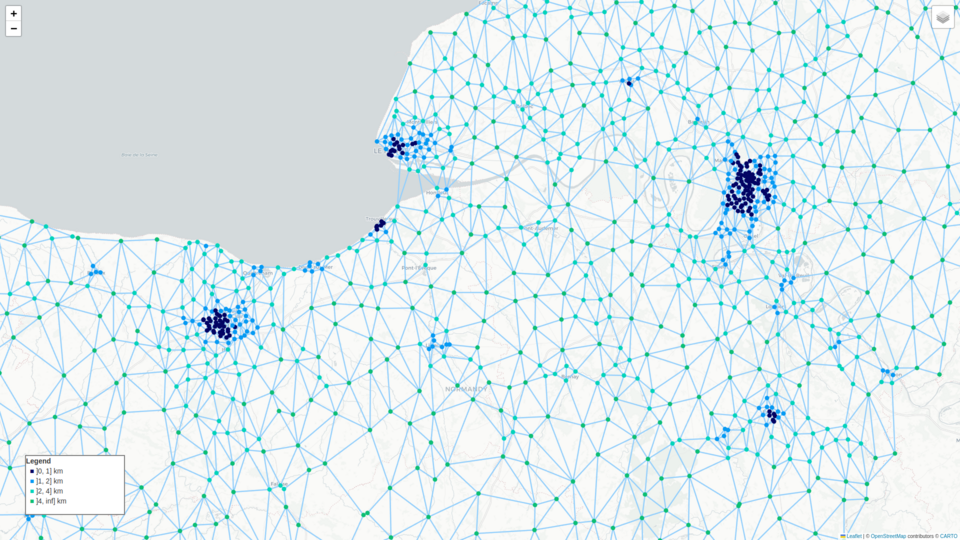
\includegraphics[width=3.5in]{images/illus_graphs/final_neighs_del_da.png}
            \caption{The final neighbouring graph.}
            \label{fig:final_neighs}
        \end{figure}

\section{Conclusion\label{sec:ccl}}
    [Ouverture: prendre en compte les zazimuths]

\bibliographystyle{IEEEtran}
\bibliography{./biblio.bib}

\end{document}